\DiaryEntry{Binomial Distribution with Beta prior}{2019-06-07}{Stochastic}

We have a Binomial distribution 

\bee
P(y=k) = {n \choose k} p^k (1-p)^{n-k}
\eee

For fun and completeness, let us calculate the maximum-likelihood estimator of $p$ (given $n$ and $k$). We differentiate $P$ wrt to $p$ and set the derivative to zero,

\bee
\frac{dP}{dp} = {n \choose k} k p^{k-1} (1-p)^{n-k} + {n \choose k} p^k (-1) (1-p)^{n-k-1} = 0
\eee

Simplifying yields

\begin{align*}
k p^{k-1} (1-p)^{n-k} - p^k (1-p)^{n-k-1} & = 0 \\
k(1-p) - (n-k)p &= 0 \\
\rightarrow p &= \frac{k}{n}
\end{align*}

This makes intuitively sense as we divide the number of successes $k$ versus the total number of observations, $n$ to get the probability of success, $p$.

\subsection{Beta Distribution}

The Beta distribution of a RV $X$ is defined on $X \in [0,1]$, has two parameters $\alpha, \beta$, and is given by

\bee
P(X = x) = \frac{x^{\alpha-1} (1-x)^{\beta-1}}{B(\alpha, \beta)}
\eee

where $B(\alpha, \beta)$ is the Beta function (see also entry \ref{2016-03-30:entry}) which normalizes the pdf; the Beta function is defined exactely this way,

\bee
B(\alpha, \beta) = \int_0^1 x^{\alpha-1} (1-x)^{\beta-1} dx
\eee

Depending on $\alpha, \beta$, the Beta distribution can take on a variety of different shapes. We first show plots for $\alpha=0.3, \beta=0.8$ (blue), $\alpha=0.8, \beta=0.3$ (red), and $\alpha=0.5, \beta=0.5$ (green).

\begin{figure}[hbt!]
\centering
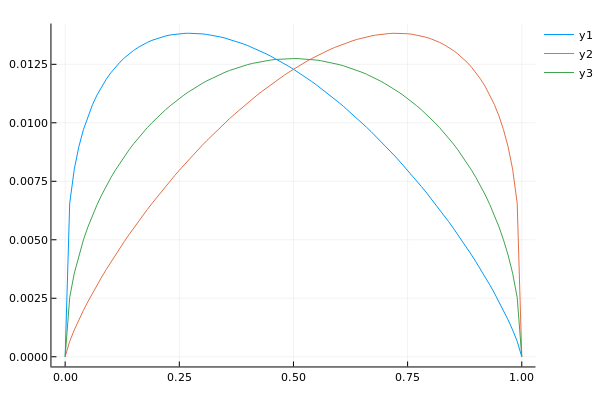
\includegraphics[scale=0.5]{images/beta_dist_1.png}
\end{figure}

Plots for $\alpha=1.3, \beta=2.5$ (blue), $\alpha=0.3, \beta=1.8$ (red) are shown in the following Figure.

\begin{figure}[hbt!]
\centering
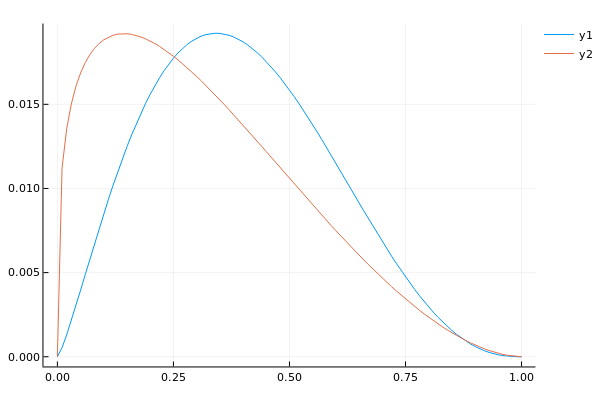
\includegraphics[scale=0.5]{images/beta_dist_2.png}
\end{figure}



We next calculate the mean,

\bee
E(X) = \int_0^1 x \frac{x^{\alpha-1} (1-x)^{\beta-1}}{B(\alpha, \beta)} dx = \frac{1}{B(\alpha, \beta)} \int_0^1 x^{\alpha} (1-x)^{\beta-1} dx = \frac{B(\alpha+1, \beta)}{B(\alpha, \beta)} 
\eee

We can insert the definition of the Beta function, $B(\alpha, \beta) = \frac{B(\alpha) B(\beta)}{B(\alpha+\beta)}$ and obtain

\bee
E(X) = \frac{ \frac{\Gamma(\alpha+1) \Gamma(\beta)}{\Gamma(\alpha+\beta+1)} }{ \frac{\Gamma(\alpha) \Gamma(\beta)}{\Gamma(\alpha + \beta)} } = \frac{\Gamma(\alpha+1) \Gamma(\alpha+\beta)}{\Gamma(\alpha) \Gamma(\alpha+\beta+1)} = \frac{\alpha}{\alpha + \beta}
\eee

where we have used the (defining) property of the Gamma function $\Gamma(x+1) = x \Gamma(x)$. \qed


What (additionally) makes the Beta distribution interesting is that it is the conjugate prior to the Bernoulli distribution; i.e. a Bernoulli distribution with $p$ distributed according to a  Beta distribution.

We observe a Bernouli RV $Y=k$ and are interested in the posterior pdf 

\bee
f(p|Y=k) = \frac{P(y | p) f(p)}{P(Y=k)} = \frac{{n \choose k} p^k (1-p)^{n-k} \frac{p^{\alpha-1} (1-p)^{\beta-1}}{B(\alpha, \beta)} }{P(Y=k)}
\eee

We first tackle $P(Y=k)$,

\begin{align*}
P(Y=k) = \int_p {n \choose k} p^k (1-p)^{n-k} \frac{p^{\alpha-1} (1-p)^{\beta-1}}{B(\alpha, \beta)} dp &= {n \choose k} \frac{1}{B(\alpha, \beta)} \int_p p^{k + \alpha-1} (1-p)^{n-k+\beta-1} dp \\
&= {n \choose k} \frac{ B(k + \alpha, n-k+\beta) }{B(\alpha, \beta)}
\end{align*}

and inserting into $f(p|Y=k)$ yields

\bee
f(p|Y=k) = \frac{{n \choose k} p^k (1-p)^{n-k} \frac{p^{\alpha-1} (1-p)^{\beta-1}}{B(\alpha, \beta)} }{ {n \choose k} \frac{ B(k + \alpha, n-k+\beta) }{B(\alpha, \beta)} } = \frac{1}{B(k + \alpha, n-k+\beta} p^{k+\alpha-1} (1-p)^{n-k+\beta-1}
\eee

This is a Beta distribution with parameters $k+\alpha, n-k+\beta$. The MMSE estimator is the mean of $f(p|Y=k)$ and therefore

\bee
\hat p_{\text{MMSE}} = \frac{k + \alpha}{n + \alpha + \beta}
\eee

We used Turing.jl to obtain an MCMC estimate of $p$ (given parameters $\alpha=0.4, \beta=1.0$ and observation $k=2$): The simulation yields 

\begin{verbatim}
 Row  parameters  mean      std      naive_se  mcse        ess     r_hat  
      Symbol      Float64   Float64  Float64   Float64     Any     Any    

 1    p           0.209182  0.1154   0.001154  0.00295325  1274.4  0.9999 
\end{verbatim}

whereas the anayltcial result yields $\hat p_{\text{MMSE}} \approx 0.2105$.

%%% Local Variables:
%%% mode: latex
%%% TeX-master: "journal"
%%% End:
